%%%%%%%%%%%%%%%%%%%%%%%%%%%%%%%%%%%%%%%%%
% Engineering Calculation Paper
% LaTeX Template
% Version 1.0 (20/1/13)
%
% This template has been downloaded from:
% http://www.LaTeXTemplates.com
%
% Original author:
% Dmitry Volynkin (dim_voly@yahoo.com.au)
%
% License:
% CC BY-NC-SA 3.0 (http://creativecommons.org/licenses/by-nc-sa/3.0/)
%
% Modificaciones por Roberto Cerdas
%
% Si desea utilizar notas al margen, favor leer los comentarios en las líneas 32 y % 52. Si desea colocar un logo, favor leer comentario en línea 54. El comando     % \marginnote{texto} introduce notas al margen.  
%
%%%%%%%%%%%%%%%%%%%%%%%%%%%%%%%%%%%%%%%%%

%----------------------------------------------------------------------------------------
%	PACKAGES AND OTHER DOCUMENT CONFIGURATIONS
%----------------------------------------------------------------------------------------

\documentclass[12pt,a4paper]{article} % Use A4 paper with a 12pt font size - different paper sizes will require manual recalculation of page margins and border positions

\usepackage[spanish]{babel} % Utilizar reglas de idioma español
\usepackage[utf8]{inputenc} % Use UTF-8 encoding
\usepackage{marginnote} % Required for margin notes
\usepackage{wallpaper} % Required to set each page to have a background
\usepackage{lastpage} % Required to print the total number of pages
%\usepackage[left=1.3cm,right=4.6cm,top=1.8cm,bottom=4.0cm,marginparwidth=3.4cm]{geometry} % Comentar la línea abajo y descomentar esta para usar notas al margen
\usepackage[left=1.3cm,right=1.3cm,top=1.8cm,bottom=4.0cm]{geometry} % Adjust page margins
\usepackage{amsmath} % Required for equation customization
\usepackage{amssymb} % Required to include mathematical symbols
\usepackage{xcolor} % Required to specify colors by name
\usepackage[square, comma, sort&compress]{natbib} % Use the natbib reference package - read up on this to edit the reference style; if you want text (e.g. Smith et al., 2012) for the in-text references (instead of numbers), remove 'numbers' 

\usepackage{fancyhdr} % Required to customize headers
\setlength{\headheight}{80pt} % Increase the size of the header to accommodate meta-information
\pagestyle{fancy}\fancyhf{} % Use the custom header specified below
\renewcommand{\headrulewidth}{0pt} % Remove the default horizontal rule under the header

\setlength{\parindent}{0cm} % Remove paragraph indentation
\newcommand{\tab}{\hspace*{2em}} % Defines a new command for some horizontal space

\newcommand\BackgroundStructure{ % Command to specify the background of each page
\setlength{\unitlength}{1mm} % Set the unit length to millimeters

\setlength\fboxsep{0mm} % Adjusts the distance between the frameboxes and the borderlines
\setlength\fboxrule{0.5mm} % Increase the thickness of the border line
\put(10, 10){\fcolorbox{black}{white!10}{\framebox(192,247){}}} % Main content box
%\put(165, 10){\fcolorbox{black}{blue!10}{\framebox(37,247){}}} % Margin box: Descomentar para utilizar notas al margen.
\put(10, 262){\fcolorbox{black}{white!10}{\framebox(192, 25){}}} % Header box
%\put(143, 263){\includegraphics[height=23mm,keepaspectratio]{logo}} % Logo box - maximum height/width: 25x42. Descomentar esta línea para usar logo.
}

%----------------------------------------------------------------------------------------
%	HEADER INFORMATION
%----------------------------------------------------------------------------------------

\fancyhead[L]{\begin{tabular}{l r | l r} % The header is a table with 4 columns
\textbf{Proyecto} & Diseño función lógica CMOS & \textbf{Página} & \thepage/\pageref{LastPage} \\ % Project name and page count
\textbf{Trabajo} & Proceso de diseño & \textbf{Actualizado en:} & 08/10/2015 \\ % Job number and last updated date
\textbf{Curso} & VLSI & \textbf{Revisado en:} & 09/10/2015 \\ % Version and reviewed date
\textbf{Diseñador} & López F. - Quirós.J.& \textbf{Revisado por:} & Alfonso Chacón Rodríguez \\ % Designer and reviewer
\end{tabular}}

%----------------------------------------------------------------------------------------

\begin{document}

\AddToShipoutPicture{\BackgroundStructure} % Set the background of each page to that specified above in the header information section

%----------------------------------------------------------------------------------------
%	DOCUMENT CONTENT
%----------------------------------------------------------------------------------------


\section{Resumen.} 

En este documento se presentan los cálculos de los tiempos de propagación y contaminación de la compuerta compuesta
\textit{F=(A+B)(C+D)}, obteniendo estos tiempos de manera analítica, mediante la teoría de esfuerzo lógico y la aproximación de Elmore, así como mediante simulación, utilizando los software \textit{Electric} y \textit{LTSpice}, y por último contrastando los resultados de ambos métodos. Tambien se muestra el diseño de un trazado que usa una única tira de difusión en ambos pozos, construyendo los \textit{caminos de Euler}, y dibujando el diagrama de palitos que muestra el orden de entradas, poly, las difusiones \textit{n} y \textit{p}, el pozo y las líneas de metal.

\section{Introducción.} 

Para el diseño de una compuerta de lógica CMOS o un conjunto de las mismas, es necesario tomar varias consideraciones para los anchos de canal de los transistores, ya sean para una optimización en potencia o para una rápida conmutación entre los niveles lógicos. En estos se debe incluir la carga que debe soportar  para que los tiempos de retardo no afecten el comportamiento ideal del circuito.

Para la demostración de los pasos de diseño de una función lógica, se nos ha pedido diseñar el esquemático y el layout de la función lógica del problema 9.4 de [1] que es \textit{F=(A+B)(C+D)}. El esquemático deberá realizarse con lógica CMOS estática.

Luego se procederá a calcular el retardo de propagación y contaminación que presenta la función, tanto de manera analítica con la aproximación de Elmore como con la teoría de esfuerzo lógico, que se evaluará con una simulación en los software \textit{Electric} y \textit{LTSpice} para saber si con este método se puede llegar a una aproximación bastante certera de los tiempos de retardo.

Por último, se realizada el layout del circuito y se volverá a realizar la simulación para definir los pitch que se usarán en la proxima tarea.

\section{Resultados Experimentales.}


\subsection{Diseño del trazado de una Compuerta y Diagrama de Palitos.}

\subsubsection{Parte 1}




\begin{table}\label{table:Tabla_polarizacion}
\begin{center}
\begin{tabular}{c||c||c||c}
Numero & Rango entrada & Región PMOS & Región NMOS\\
\hline
\hline
1 & $V_{in}<V_{tn}$ & Lineal & Corte \\
2 & $V_{tn}<=V_{in}<V_{inv}$ & Lineal & Saturación \\
3 & $V_{in}=V_{inv}$ & Saturación & Saturación\\
4 & $V_{inv}<V_{in}<=V_{dd}+V_{tp}$ & Saturación & Lineal\\
5 & $V_{in}>V_{dd}+V_{tp}$ & Corte & Lineal\\
\hline
\end{tabular}
\caption{Regiones inversor CMOS Vin vs Vout}
\end{center}
\end{table}


\begin{figure}[htbp]
  \centering
    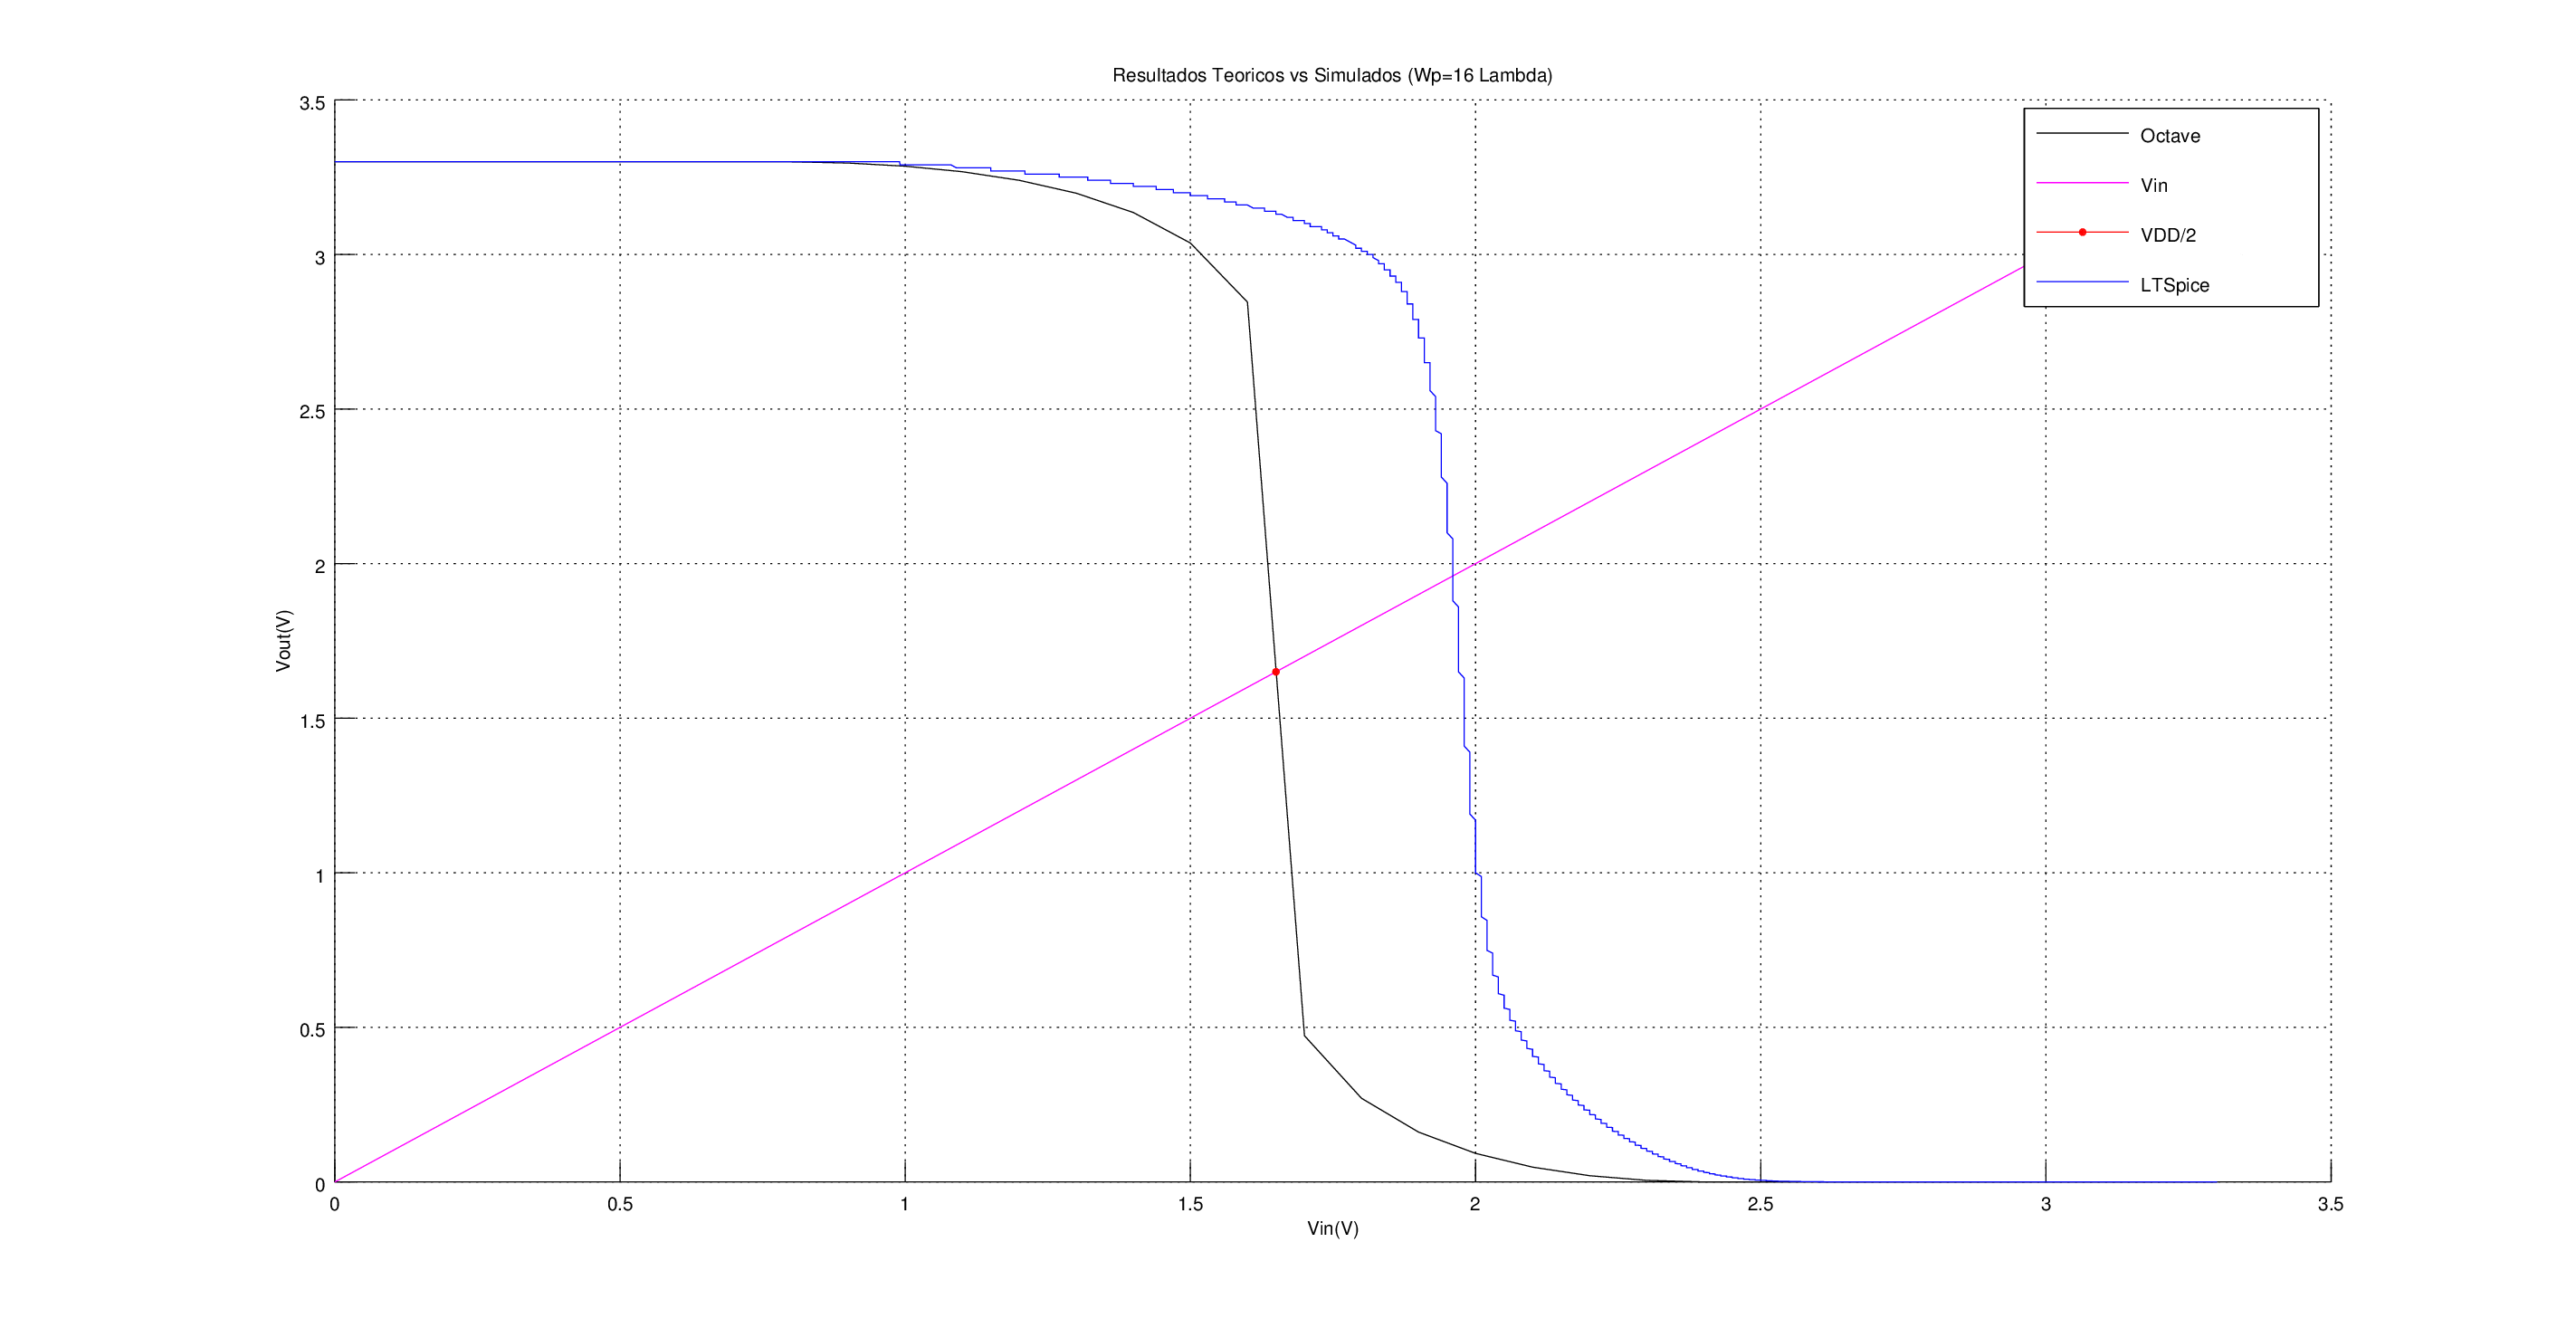
\includegraphics[scale=0.2]{./Inv_16lam.png}
    \rule{35em}{0.5pt}
  \caption[IdealvsSim]{Graficas \textit{Octate} Ideal vs Simulacion \textit{Electric}}
  \label{fig:inv_est}
\end{figure}

Para la simulación experimental, se usó el programa \textit{Electric}. En esta simulación se utilizó el archivo \textit{Mosis\_5} para las constantes de la tecnología MOSIS 0.5. Ya realizada la simulación del inversor (fig.\ref{fig:inv_est2}) con la relación de ancho de canal calculado anteriormente encontramos que la proporción de regiones en el inversor no es la esperada, por lo que se decidió volver a dimensionar el ancho de los canales con respecto a las simulaciones y encontramos que de manera experimental la relación correcta es \textit{r=1.575}. 




\subsection{Delay de Propagación y de Contaminación.}

\subsubsection{Método Analítico}

El cálculo de los tiempos de propagación y de contaminación se realiza haciendo uso de dos métodos: la teoría del esfuerzo lógico, \textit{logical effort}, y por el método de la aproximación de Elmore, \textit{Elmore Delay}.\\

\subsubsection{Método de Esfuerzo Lógico}

El esfuerzo lógico se define como \textit{"la razón de la capacitancia del gate a la capacitancia de entrada de un inversor que puede entregar la misma corriente de salida."}, e indica que tan mala es una compuerta produciendo una corriente de salida comparada con un inversor.\\

Para el cálculo del delay por medio de la teoría de esfuerzo lógico, se utilizan las formulas del calculo del delay en redes lógicas multi-etapa, \textit{Multistage Logical Network}, que utiliza las siguientes formulas pára el cálculo del delay:\\

\begin{equation}\label{eqn:esfuerzo_logico}
G= \prod g_{i}
\end{equation}

\begin{equation}\label{eqn:esfuerzo_electrico}
H= \frac{C_{out-path}}{C_{in-path}}
\end{equation}

\begin{equation}\label{eqn:esfuerzo_enramado}
B= \prod b_{i}
\end{equation}

\begin{equation}\label{eqn:esfuerzo}
F = GBH
\end{equation}

\begin{equation}\label{eqn:delay_parasitico}
P = \sum p_{i}
\end{equation}

\begin{equation}\label{eqn:delay}
D = NF^{\frac{1}{N}} + P
\end{equation}

En donde \textit{G} es el esfuerzo lógico, \textit{H} es el esfuerzo eléctrico, \textit{B} el esfuerzo de enramado, \textit{F} es el esfuerzo total, \textit{P} es el delay parasítico del camino, \textit{N} es la cantidad de estapas del camino y \textit{D} es el delay total del camino.\\

La función \textit{F=(A+B)(C+D)} se puede representar a nivel de compuerta como se muestra en la fig.\ref{fig:OAI21} , donde se observa que la compuerta es del tipo OR-OR-AND-INV + INVERSOR, \textit{OAI-21 + inverter}, y a partir de aqui se calcula el esfuerzo lógico de camino.\\

\begin{figure}[htbp]
  \centering
    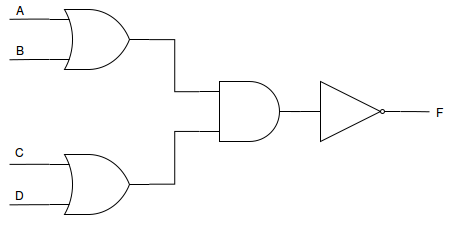
\includegraphics[scale=0.5]{./OAI21.png}
    \rule{35em}{0.5pt}
  \caption[IdealvsSim]{Compuerta \textit{OAI-21}.}
  \label{fig:OAI21}
\end{figure}\\

Para realizar los cálculos del esfuerzo de camino de esta función, se debe tomar en cuenta que cada entrada presenta como maximo 30$\lambda$ de ancho de transistor, y que la salida debe de manejar una carga equivalente de 500$\lambda$ de ancho de transistor, como se muestra en la fig.\ref{fig:OAI21_Cargas}. Se puede observar que en este caso el número de etapas, \textit{N}, es igual a 2, por lo que haciendo uso de las ecuaciones \ref{eqn:esfuerzo_logico}, \ref{eqn:esfuerzo_electrico}, \ref{eqn:esfuerzo_enramado}, \ref{eqn:esfuerzo}, \ref{eqn:delay_parasitico}, \ref{eqn:delay}, se puede encontrar el delay mediante la teoría de esfuerzo lógico de cada entrada bajo estas condiciones de carga.\\

\begin{figure}[htbp]
  \centering
    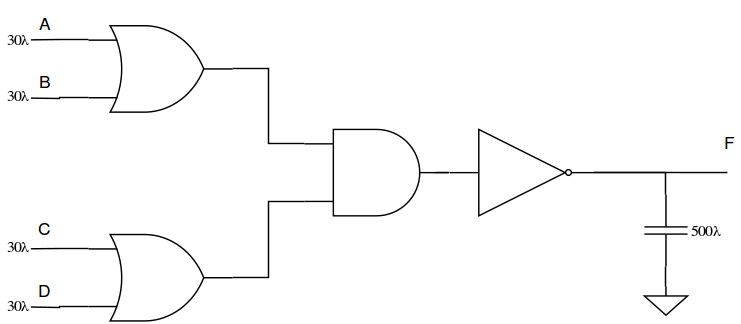
\includegraphics[scale=0.5]{./OAI21_Cargas.png}
    \rule{35em}{0.5pt}
  \caption[IdealvsSim]{Compuerta \textit{OAI-21} con carga.}
  \label{fig:OAI21_Cargas}
\end{figure}\\


\begin{equation}\label{eqn:esfuerzo_logico2}
G= \prod g_{i}= \frac{6}{3} * 1 = \frac{6}{3}
\end{equation}

\begin{equation}\label{eqn:esfuerzo_electrico2}
H= \frac{C_{out-path}}{C_{in-path}} = \frac{500\lambda}{30\lambda} = \frac{50}{3}
\end{equation}

\begin{equation}\label{eqn:esfuerzo_enramado2}
B= \prod b_{i} = 1
\end{equation}

\begin{equation}\label{eqn:esfuerzo2}
F = GBH = \frac{6}{3}*1*\frac{50}{3} = \frac{100}{3}
\end{equation}

\begin{equation}\label{eqn:delay_parasitico2}
P = \sum p_{i} = \frac{12}{3} + 1 = \frac{15}{3} = 5
\end{equation}

\begin{equation}\label{eqn:delay2}
D = NF^{\frac{1}{N}} + P = 2*(\frac{100}{3})^{\frac{1}{2}} + 5 = 16.54\tau
\end{equation}\\

El cálculo de los tiempos arroja como resultado que cada entrada de esta compuerta tendrá un delay de \textit{16.54$\tau$}.\\

Con el valor de delay calculado se puede proceder a dimensionar los transistores que conforman la compuerta. En la fig.\ref{fig:Comp_Transistores} se muestra la compuerta compuesta a nivel de transistores, sin dimensionar.\\

\begin{figure}[htbp]
  \centering
    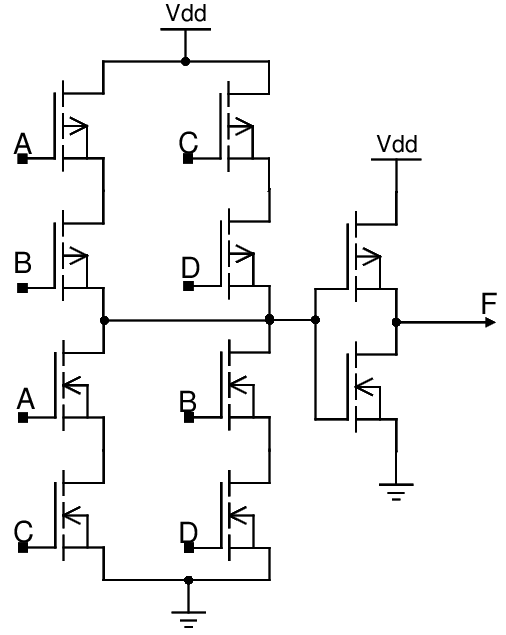
\includegraphics[scale=0.5]{./Comp_Transistores.png}
    \rule{35em}{0.5pt}
  \caption[IdealvsSim]{Compuerta \textit{OAI-21} con carga.}
  \label{fig:Comp_Transistores}
\end{figure}\\

Para dimensionar los transistores de cada entrada, se toma en cuenta el modelo RC del transistor. Sabiendo que la resitencia de la red \textit{PMOS} debe ser igual a la de la red \textit{NMOS}, y que cada entrada presenta como maximo 30$\lambda$ de ancho de transistor se obtiene que:\\

\begin{equation}\label{eqn:R}
\frac{2R}{k_p} = \frac{R}{k_n}
\end{equation}

\begin{equation}\label{eqn:k}
k_p + k_n = 30\lambda
\end{equation}\\

Donde \textit{$k_{p}$} y \textit{$k_{n}$} son los anchos de los tansistores p y n de cada entrada. Con este sistema de ecuaciones se obtiene que:

\begin{equation}\label{eqn:R1}
k_p = 2k_n
\end{equation}

\begin{equation}\label{eqn:k1}
k_p + k_n = 30\lambda
\end{equation}

\begin{equation}\label{eqn:k2}
3k_n = 30\lambda
\end{equation}

\begin{equation}\label{eqn:k3}
k_n = 10\lambda ; k_p = 20\lambda
\end{equation}\\

Utilizando la ec.\ref{eqn:k_Inv}, se puede encontrar la capacitancia de entrada del inversor, como se muestra a continuación:\\

\begin{equation}\label{eqn:k_Inv}
{C_{in}}_{i}= \frac{C_{out}_{i}*g_{i}}{F^{\frac{1}{N}}}
\end{equation}\\


\subsubsection{Método de Aproximación de Elmore}

Ahora se calcula el delay de propagación y el delay de contaminación de la compuerta \textit{F=(A+B)(C+D)} mediante el método de \textit{Aproximación de Elmore}, el cuál se hace valer del modelo RC del transistor, para calcular los delays de una compuerta. El modelo de delay de \textit{Elmore} estima el restraso desde una fuente conmutando a uno de los nodos hoja cambiantes como la suma sobre cada nodo \textit{i} de la capacitancia \textit{$C_{i}$} en el nodo, multiplicado por la resistencia efectiva \textit{$R_{is}$} en el camino compartido desde la fuente hasta el nodo y la hoja, dando como resultado la ec.\ref{eqn:Elmore}:

\begin{equation}\label{eqn:Elmore}
t_{pd} = \sum_{i} R_{is}C_{i}
\end{equation}\\


En la fig.\ref{fig:ModeloRC_Completo} se muestra el modelo RC completo de la compuerta,
\subsubsection{Carga y descarga de un capacitor}

Para el cálculo de las resistencias de canal de cada transistor, se utilizo una capacitancia de carga y descarga de \textit{1pF}, se montaron los circuitos de las figuras \ref{fig:R_PMOS} y \ref{fig:R_NMOS} en el software \textit{Electric} y se simularon los resultados en  \textit{LTSpice}, obteniendo las curvas que se observan en las figuras \ref{fig:Grafica_R_PMOS} y \ref{fig:Grafica_R_NMOS}, para el caso de carga y descarga, respectivamente.\\

\begin{figure}[htbp]
  \centering
    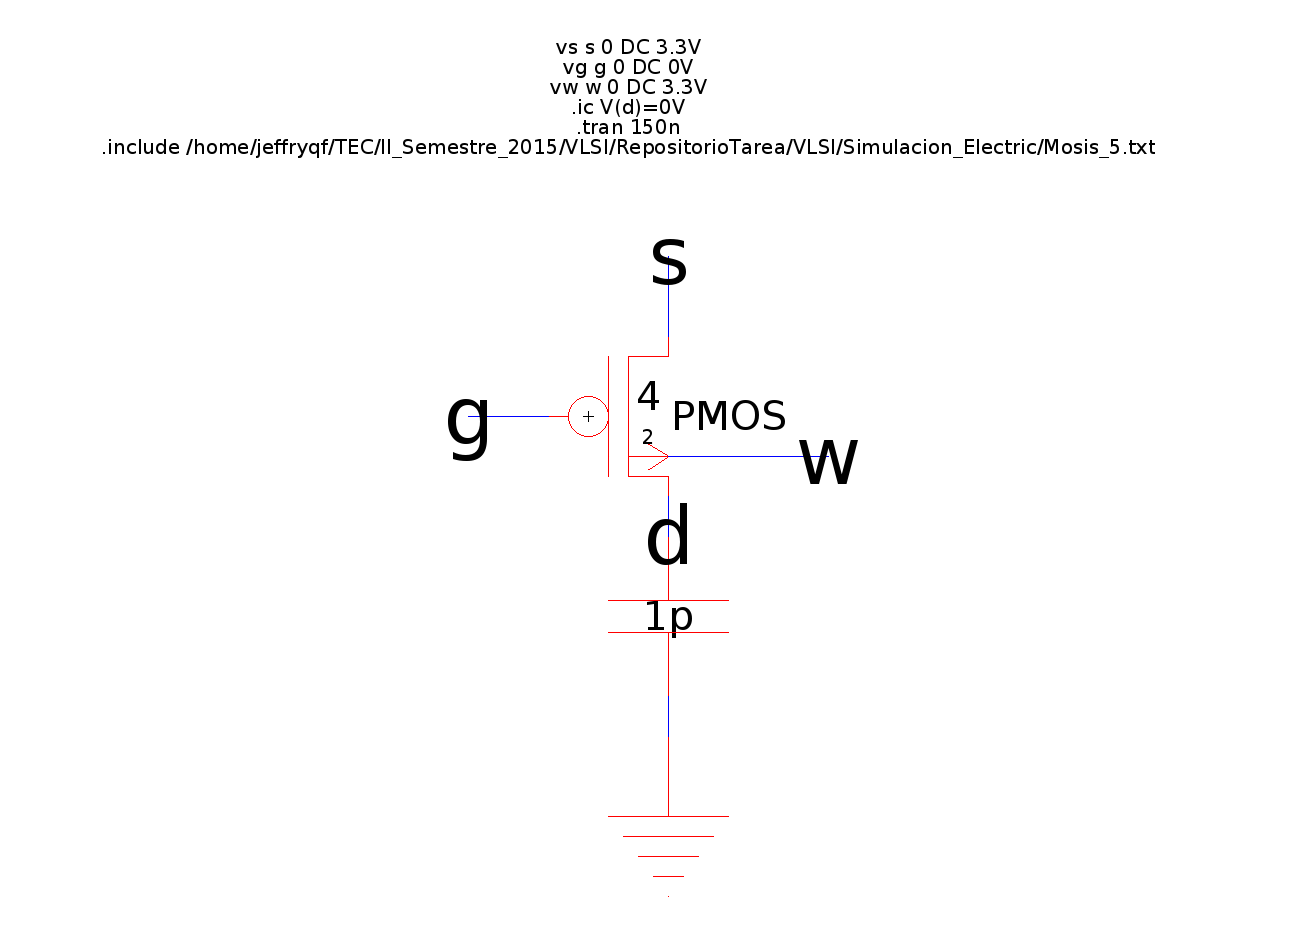
\includegraphics[scale=0.3]{./R_PMOS.png}
    \rule{35em}{0.3pt}
  \caption[C_Carga]{Circuito de Carga de Capacitor.}
  \label{fig:R_PMOS}
\end{figure}

\begin{figure}[htbp]
  \centering
  	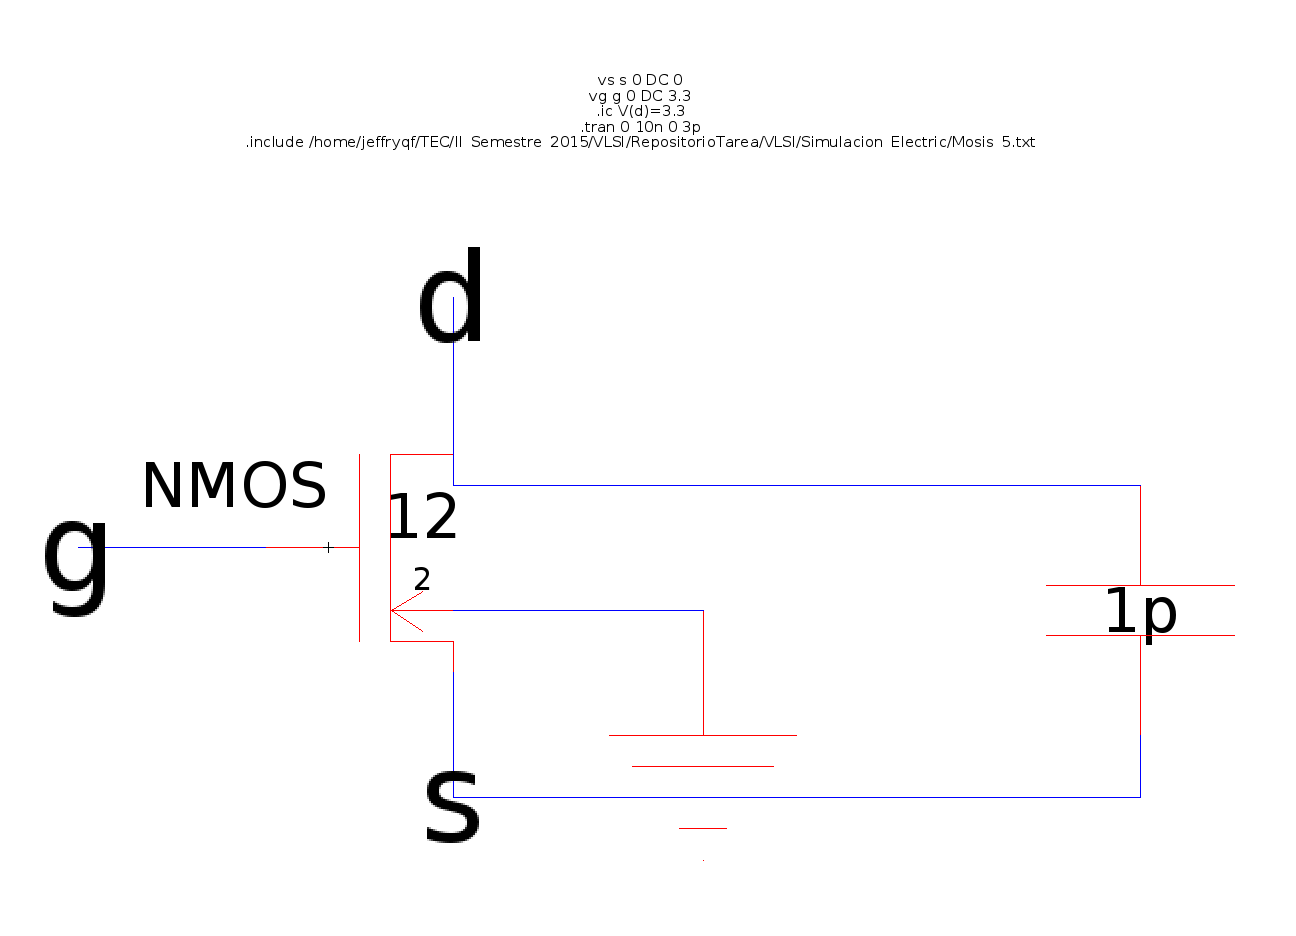
\includegraphics[scale=0.3]{./R_NMOS.png}
    \rule{35em}{0.3pt}
  \caption[C_Descarga]{Circuito de Descarga de Capacitor.}
  \label{fig:R_NMOS}
\end{figure}

\begin{figure}[htbp]
  \centering
    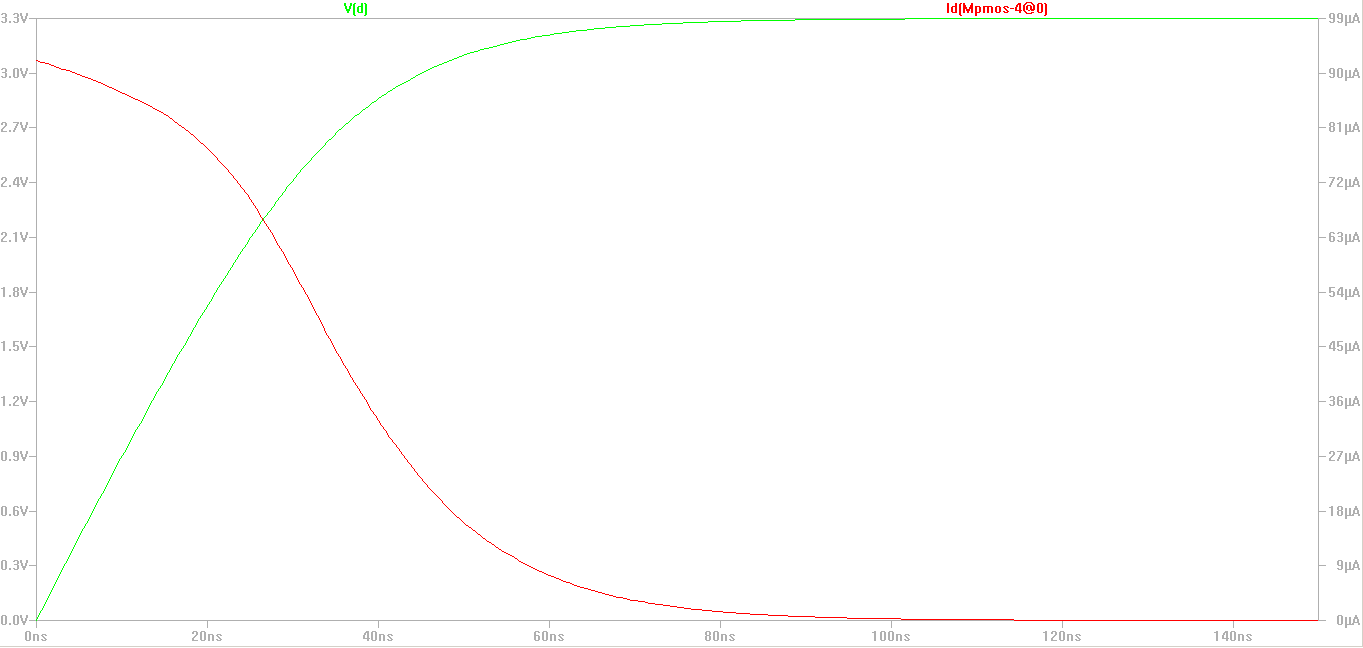
\includegraphics[scale=0.3]{./Grafica_R_PMOS.png}
   \rule{35em}{0.3pt}
  \caption[G_Carga]{Grafica de comportamiento de $\textit{I}_{\textit{d}}$ durante la carga del Capacitor.}
  \label{fig:Grafica_R_PMOS}
\end{figure}

\begin{figure}[htbp]
 \centering
    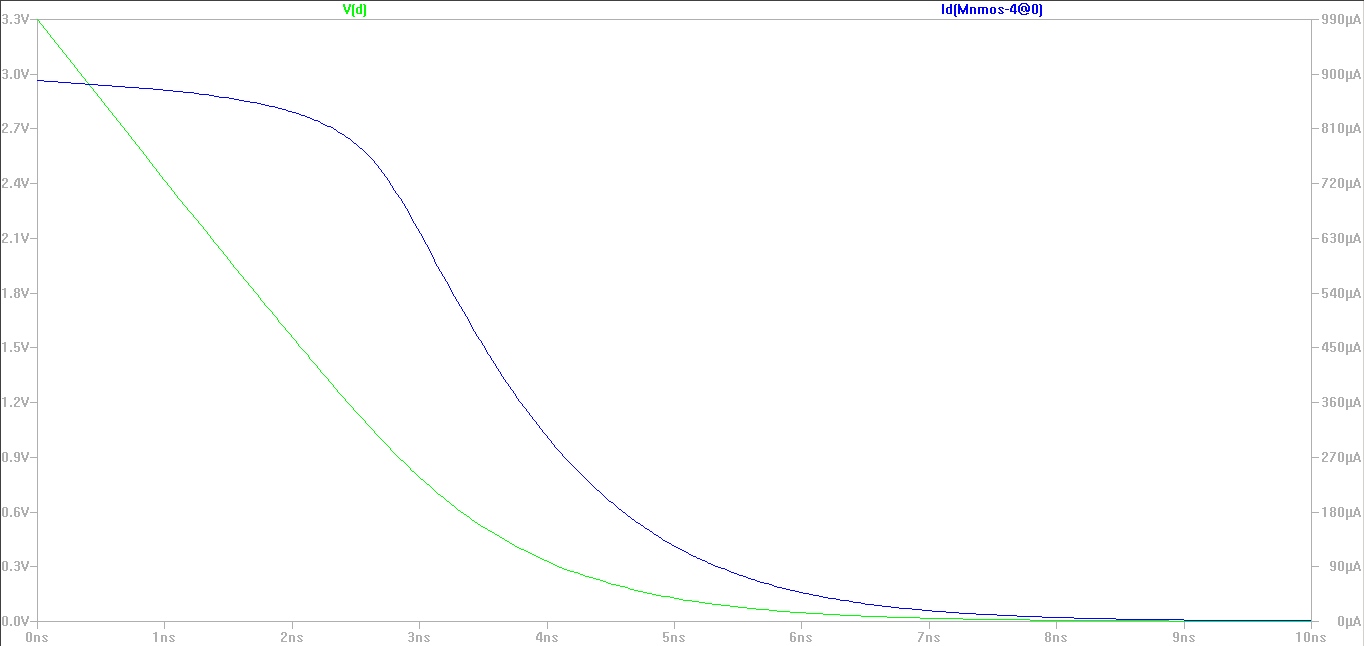
\includegraphics[scale=0.3]{./Grafica_R_NMOS.png}
    \rule{35em}{0.3pt}
  \caption[G_Descarga]{Grafica de comportamiento de $\textit{I}_{\textit{d}}$ durante la descarga del Capacitor.}
  \label{fig:Grafica_R_NMOS}
\end{figure}

Utilizando un pequeño script en \textit{Octave}, se procesan los puntos obtenidos en estas graficas y se calculan la resistencias de canal promedio de cada transistor, obteniendo los siguientes resultados:

\begin{equation}\label{eqn:R_PMOS}
Req_P = 8.7860k\Omega
\end{equation}

\begin{equation}\label{eqn:R_NMOS}
Req_N = 2.6919k\Omega
\end{equation}

\subsubsection{Método de Fanout}

El método de Fanout plantea encontrar la resistencia equivalente de un transistor \textit{CMOS} con los valores de la capacitancia parásita en el gate y el diferencial de tiempos de caída y levantamiento que le toma al mismo pasar de un nivel lógico a otro, con 2 valores de \textit{fanout} distintos. Las ecuaciones para calcular las resistencias equivalentes para \textit{PMOS} y \textit{NMOS} son las \ref{eqn:Req_p} y \ref{eqn:Req_n} respectivamente.\\*
\\*
\begin{equation}\label{eqn:Req_p}
R_{eqp}=(2/3)*( \Delta t_{r}/C_{g})
\end{equation}

\begin{equation}\label{eqn:Req_n}
R_{eqn}= \Delta t_{f}/(3*C_{g})
\end{equation}

Se realizó la simulación del circuito propuesto encontrado en la referencia [1] sección 8.4.5. , para valores de \textit{h=2} (fig. \ref{fig:CircuitoFO2}) y \textit{h=3} (fig. \ref{fig:CircuitoFO3} con los cuales se encontraron las graficas de los retardos de la salida con respecto a la entrada (fig. \ref{fig:FO2} y fig. \ref{fig:FO3})\\*
\\*
\begin{figure}[htbp]
\begin{center}
    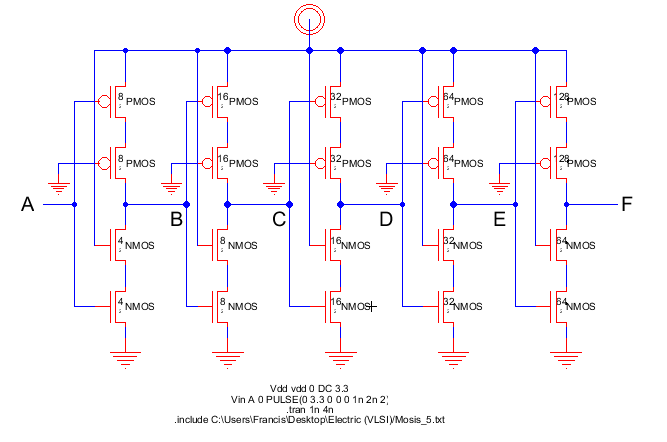
\includegraphics[scale=0.5]{./CircuitoFO2.png}
    \rule{35em}{0.5pt}
  \caption[Captura]{Circuito para calculo de $R_{eq}$ con h=2}
  \label{fig:CircuitoFO2}
  \end{center}
\end{figure}

\begin{figure}[htbp]
  \centering
    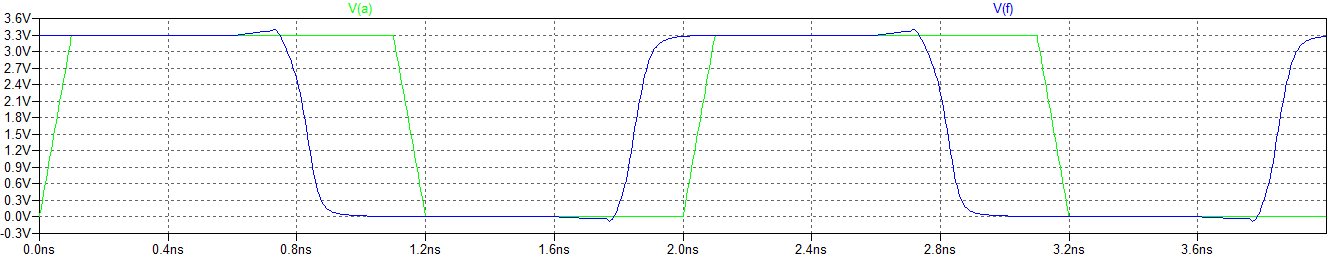
\includegraphics[scale=0.4]{./FO2.png}
    \rule{35em}{1pt}
  \caption[Captura]{Gráfica tiempo $V_{in}$ vs $V_{out}$ h=2}
  \label{fig:FO2}
\end{figure}

\begin{figure}[htbp]
\begin{center}
    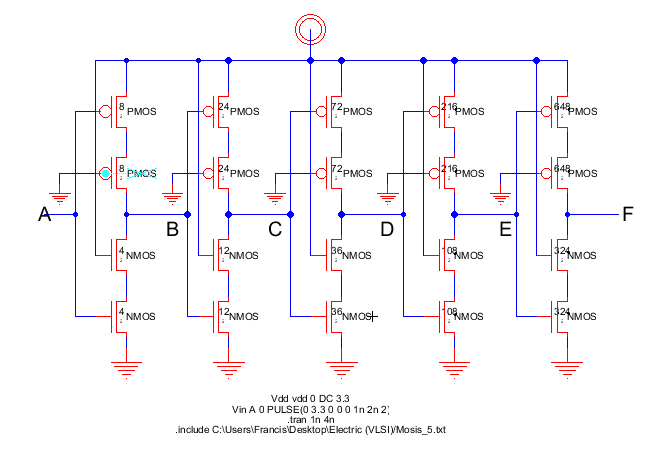
\includegraphics[scale=0.5]{./CircuitoFO3.png}
    \rule{35em}{0.5pt}
  \caption[Captura]{Circuito para calculo de $R_{eq}$ con h=3}
  \label{fig:CircuitoFO3}
  
\end{center}
\end{figure}

\begin{figure}[htbp]
  \begin{center}
    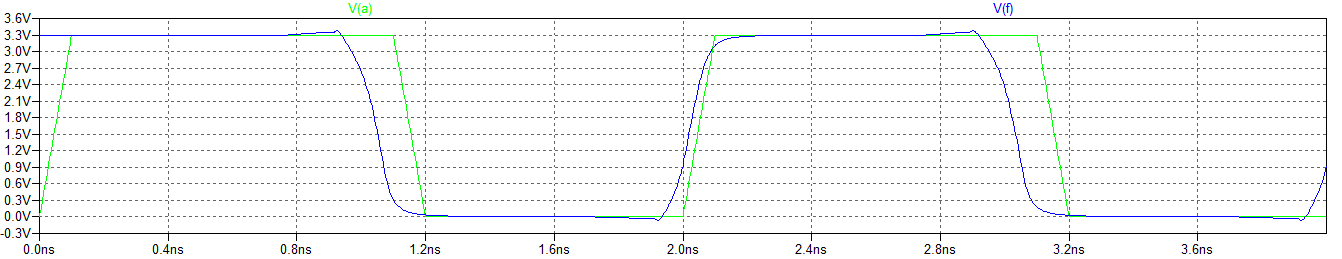
\includegraphics[scale=0.4]{./FO3.png}
    \rule{35em}{0.5pt}
  \caption[Captura]{Gráfica tiempo $V_{in}$ vs $V_{out}$ h=3}
  \label{fig:FO3}
  \end{center}
\end{figure}

Luego de encontrar las gráficas (fig. \ref{fig:FO2} y fig. \ref{fig:FO3}), se realizó la medición de los tiempos ya mencionados anteriormente. Aunque en la referencia [] se habla que la medición debe hacerse entre los valores de $0.8V_{dd}$ a $0.2V_{dd}$, se encontró que las pendientes de ambas graficas son aproximadamente iguales y no se encontraría la variación de la resistencia equivalente entre los CMOS por lo que se decidió medir de $0.9V_{dd}$ a $0.1V_{dd}$. Se encontraron los valores mencionados en el cuadro \ref{table:tiempos}. \\*
\\*
\begin{table}\label{table:tiempos}
\begin{center}
\begin{tabular}{c||c||c}
n & tr(ps) & tf(ps)\\
\hline
\hline
2 & 97.36 & 101.29 \\
3 & 117.84 & 125.055 \\
$\Delta$ & 20.44 & 23.76\\
\hline
\end{tabular}
\caption{Tiempos de levantamiento y caida de tensión para un inversor CMOS para diferentes Fanouts}
\end{center}
\end{table}


Ya con los diferenciales de tiempos medidos, se sustituyen en \ref{eqn:Req_p} y \ref{eqn:Req_n} para encontrar la resistencia equivalente de cada transistor. Para $C_{g}=1.48 fF/\mu m$  dependiente del ancho de canal de gate, se encuentra que los valores de resistencia son los del cuadro (\ref{table:resistencias}). \\*
\\*
\begin{table}\label{table:resistencias}
\begin{center}
\begin{tabular}{c||c}
Resistencia & k$\Omega$\\
\hline
\hline
$R_{eqp}$ & 15.375 \\
$R_{eqn}$ & 9.000 \\
\hline
\end{tabular}
\caption{Resistencias equivalentes encontradas por Método de Fanout}
\end{center}
\end{table}




\section{Análisis de datos y resultados.}

Los resultados obtenidos en la sección \textit{3.1.2}, muestran el diseño del ancho del canal de un transistor \textit{PMOS}, para conseguir que los tiempos de propagación sean simétricos. Los resultados obtenidos de la Ec.\ref{eqn:Beta2}, muestra un valor de relación de tamaño de ancho de canal de los transistores en un inversor de \textit{1.3070}, lo que equivale a decir que el ancho del canal del tansistor \textit{PMOS} es de 5$\lambda$, pero a la hora de simular se ajusto este valor hasta conseguir que la relación sea \textit{1.5}, esto con el fin no solo de lograr que los valores de propagación de la señal fueran simétricos, si no también para conseguir una tensión de umbral del inversor cercana a \textit{1.65V}, como se observa en la fig.\ref{fig:DC_Comp}, siendo asi entonces que el nuevo tamaño del ancho de canal del transistor \textit{PMOS} es de 6$\lambda$.\\*
\\*Uno de los resultados relevantes que pudimos encontrar del dimensionamiento del transistor \textit{PMOS} es en el hecho que las corrientes de corto circuito de la fig. \ref{fig:CC} son aproximadamente iguales, los cual nos dice que la potencia de los transistores en ambos procesos es igual. Podemos deducir que mediante un análisis dinámico para el dimensionamiento de los transistores es el método que deber usarse para el diseños de las compuertas, esto porque la símetría de las transiciones se puede obviar con respecto a tener un mínimo del tiempo de retardo para las mismas, dando como resultado, que los circuitos puedan conmutar a una mejor velocidad con la misma potencia que si se hiciese de forma simétrica las compuertas.\\*
\\*En la sección 3.2 se procede a calcular el valor de las resistencias de canal para un trasistror \textit{PMOS} y un transistor \textit{NMOS}, mediante dos métodos diferentes. \\

En la sección 3.2.1 se calculó la resistencia de canal por un método grafico, simulando la carga y descarga de un capacitor y obteniendo la curva de comportamiento de la corriente de \textit{drain} de un transistor \textit{PMOS} y \textit{NMOS}, respectivamente, y con esto obteniendo los valores de resistencia que se muestran en la Ec.\ref{eqn:R_PMOS} y Ec.\ref{eqn:R_NMOS}. Se considera que este método no es muy preciso al tratarse del cálculo de un valor a partir de una aproximación, que dependerá de la cantidad de valores muestrados y de la precisión de dichos valores, lo que dio como resultado obteniendo por ende un valor promedio de resistencia.\\*

En cambio, para la sección 3.2.2, encontramos que los valores de las resistencias equivalentes son mas precisos, por el método que se emplea y que no realiza tantas aproximaciones y suposiciones para encontrar el valor de los mismos.


\section{Conclusiones.}
\begin{itemize}
\item La ecuaciones de Shockley no da un comportamiento real de los transistores PMOS y NMOS, si no un comportamiento muy aproximado.
\item El uso de diversas herramientas de simulación nos permiten encontrar proporciones de diseño bastante precisas
\item El diseño de un inversor apropiado debe de procurar un balance entre el mejoramiento de los tiempos de propagación, asi como la obtención de una tension de umbral lo más cercana a $\textit{V}_\textit{DD}/2$.
\item El análisis de tiempos de propagación provee un mejor punto de arranque para la obtención del tamaño de un transistor \textit{PMOS}, permitiendo realizar ajustes en simulación que permitan llegar a un valor concreto de manera más rapida.
\item El método grafico para la obtención de los valores de resistencia de canal no es el mas apropiado, aunque provee una forma rapida de encontrar un valor de resistencia aproximado aceptable.
\item Se recomienda para encontrar la resistencia equivalente de los transistores el método de Fanout
\end{itemize}

%----------------------------------------------------------------------------------------
\begin{thebibliography}{3}

\bibliographystyle{unsrtnat} % Use the "unsrtnat" BibTeX style for formatting the Bibliography

\bibitem[Wey(1999)]{Wey1999}
[1] N. Weste, D. Harris. 
\newblock {CMOS VLSI Design: A Circuits and Systems Perspective , 4 edition.}.
\newblock \emph{Boston: Addison-Wesley}, 2010.

\bibitem[Wey(1999)]{Wey1999}
[2] J. Rabaey, A. Chandrakasan y B. Nikolic. 
\newblock { Digital Integrated Circuits: A Design Perspective.}.
\newblock \emph{Prentice Hall}, 2005.

\bibitem[Wey(1999)]{Wey1999}
[3]Test Data .On SemiconductorC5.Mosis. Recompilado de:
\newblock \emph{http://www.ie.itcr.ac.cr/achacon/ \\* Intro$\_$Diseno$\_$CI/Modelos$\_$Spice$\_$MOSIS/v03m-params.txt}, el 07/09/2015

\end{thebibliography}

\end{document}